The purpose of this section is to give a detailed schematic of our optical table setup. The setup is divided into two parts, a pre-setup part describing how we manipulate the cavity input and lock the laser to the cavity and a second part including the cavity and detection scheme. It should be noted that three persons have simultaneously been working on the setup, so the setup is constantly being altered to fit the current workloads. We begin with the pre-setup shown in figure \ref{fig:presetup}.

\begin{figure}[H]
\centering
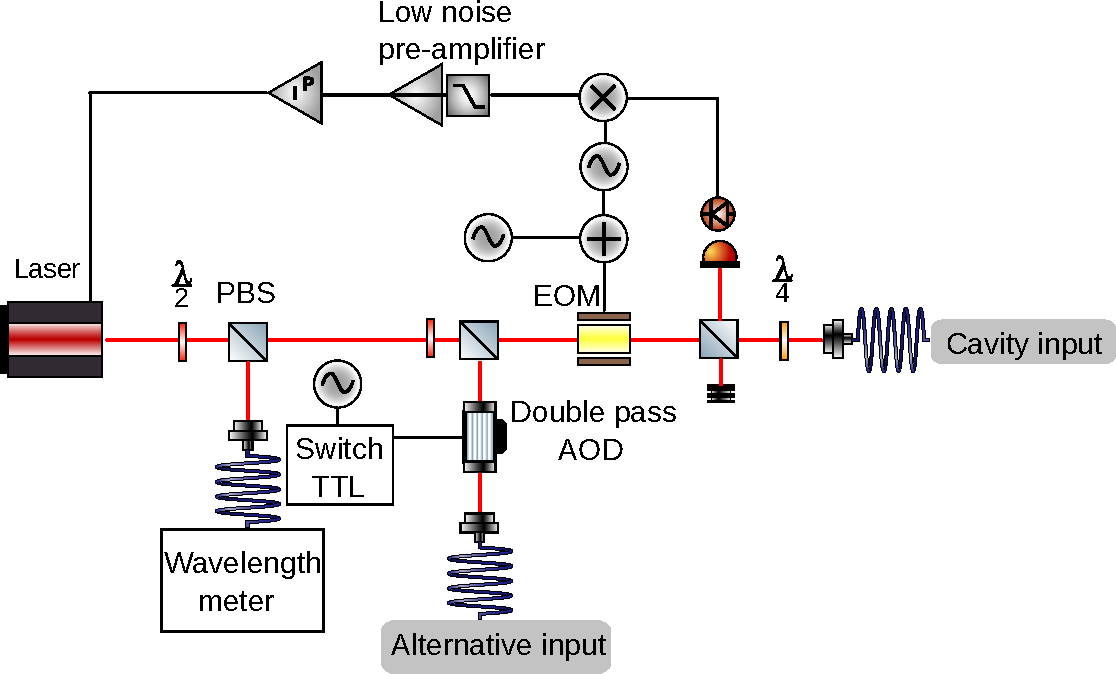
\includegraphics[scale=0.8]{setup.pdf}
\caption{Detailed overview of the pre-setup on our optical table.}
\label{fig:presetup}
\end{figure}

\subsection{Input}
The laser used is a narrow linewidth widely tunable CW titanium sapphire (Ti:sapphire)\footnote{MSquared SolsTiS}. It has the special property of having a low phase noise and a low relative intensity noise for the frequencies we want to work at, meaning that we are shot noise limited at roughly \SI{1}{\mega\hertz} and upwards (see appendix \ref{sec:rin}). The laser comes with commercial control software for tuning/scanning the wavelength and locking it to its external reference cavity for stability. It can be operated with a wavelength in the range 725-975 \SI{}{\nano\meter} and it has a narrow linewidth of \SI{18}{\kilo\hertz} if locked to its reference cavity.

The laser light enters the pre-setup and is directly split into two beams by a half wave plate ($\lambda/2$) and polarizing beam splitter (PBS). Most of the optical power is transmitted through the PBS. The reflected beam is fiber coupled and sent to a Bristol 521-NIR wavelength meter which has an accuracy of \SI{\pm 10}{pm}, since the built-in commercial wavelength meter in the laser is not accurate enough $\pm 100$ pm. The Bristol wavelength meter is then connected to a computer, where we read off the wavelength.

\subsection{Primary input}
The transmitted beam after the first PBS is split again by a $\lambda/2$-plate and a PBS. The transmitted beam is sent to a fiber coupled \SI{10}{\giga\hertz} electro-optical-modulator\footnote{EOSpace PM-0K1-10-PFU-PFU-850-UL-S} (EOM), which takes two inputs from signal generators to generate a sideband for the locking scheme as wel as one for sweeping a probe field across the cavity resonance. The output from the EOM is sent through a PBS and a quarter wave plate ($\lambda/4$) and then fiber coupled and sent as primary input to the cavity. The $\lambda/4$-plate and PBS is in reality a three armed fiber coupled beam splitter, which sends the cavity reflection to a fiber coupled photodetector\footnote{Thorlabs PDA8GS}. For illustrative reasons it is pictured as a wave plate and a PBS. The detector in reflection is used to both set up a Pound-Drever-Hall lock \cite{black2001}, and as a tool for optimizing backreflection from the flat bottom mirror during the assembly procedure. For the lock feedback we use a low noise pre-amplifier\footnote{Stanford Research Systems SR560} and a commercial servo box\footnote{New Focus LB1005 Servo Controller}. We do not use the PDH lock for the experiments presented here, so the error signal is then taken from the transmission detector.

\subsection{Alternative input}
The reflected beam of the PBS in the middle is sent to a double-pass \SI{120}{\mega\hertz} acuosto-optic deflector\footnote{IntraAction corp. ATD-1202DA2} (AOD) setup, such that we can modulate without misaligning the beam path. The AOD is driven by a signal generator connected to a home-built TTL switch board. This alternative input serves the purpose of optically exciting the membrane's mechanical modes, as will be explained in detail in section \ref{sec:q_fact}.

\subsection{Cryo-cavity and detection}
In the lab lingo, we often refer to our setup as the cryo-cavity setup and now the name has also found its way into this work. See figure \ref{fig:cryocavity} for a detailed overview. The fiber from pre-setup is attached on a fiber output-coupler, where tilt/angle can be adjusted. The output-coupler is placed on a XYZ-stage. These degrees of freedom are crucial for alignment of the cavity, fixing membrane mirror tilt and optimizing optomechanical coupling. Right after the the coupler a lens ($f = $\SI{11}{\milli\meter}) is placed to mode match the wave fronts to the cavity. The transmission from the cavity is then put on a 92:8 beamsplitter, where the reflected beam is sent to a camera\footnote{Mightex} and the transmitted beam is put on a photodetector\footnote{Thorlabs APD110A}. The detector signal is split into a DC part and RF part by a Bias Tee\footnote{Mini Circuit ZF8T-4R2G} with a cuf-off frequency of \SI{10}{\mega\hertz}. The DC part of the signal is then sent to an oscilloscope and RF part is sent to a network analyzer or sometimes just a spectrum analyzer depending on the situation. For the work presented in here we setup the lock using the transmission detector for a simple slope lock, which will be described in section \ref{sec:exp_omit}.

\begin{figure}[H]
\centering
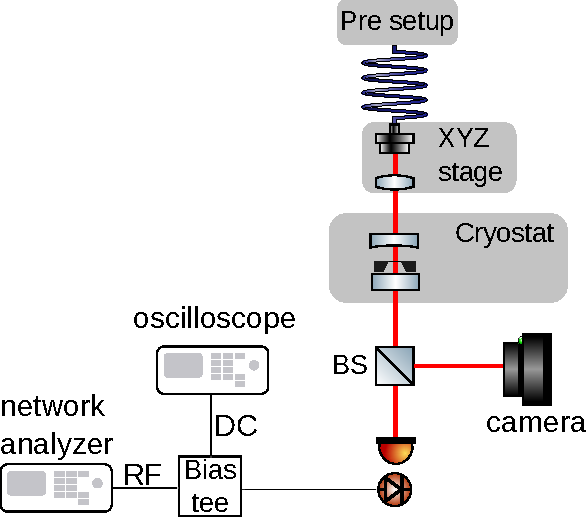
\includegraphics[scale=1.1]{cryocavity.pdf}
\caption{Cryo-cavity setup.}
\label{fig:cryocavity}
\end{figure}